
\chapter{Overzicht planning en fases}
\label{app:planning}

In de volgende twee pagina's zijn de planning en fases in meer detail omschreven\footnote{ Deze pagina's zijn in het engels geschreven, omdat dit de voertaal is binnen het bedrijf }. De onderzoekmethode, zie tabel \ref{tab:onderzoekmethode} op pagina \pageref{tab:onderzoekmethode}, dient als basis voor deze planning.
\newline

In de "Breakdown structrure, estimates per activity"\ wordt inzichtelijk gemaakt hoe de tijd is onderverdeeld per activiteit en Proof of concept. Er wordt rekening gehouden met de mogelijke risico's en daarom kan in werkelijkheid de uitvoering sneller dan hier ingepland.

In de lijst met lijst met activiteiten, zie sectie \ref{sec:activiteiten} op pagina \pageref{sec:activiteiten}, zijn de inschattingen in uren geschreven. Echter zijn de inschattingen origineel gedaan in dagen, omdat dit beter aansluit bij de werkwijze van Shop2market. Dit wordt dan ook gehanteerd in apendix \label{app:planning}.
\newline

In "Visualisation in calendar days based on estimates per activity"\ is te zien hoe de planning past binnen de iteraties bij Shop2market, aansluitend bij de werkwijze in de organisatie. Andere belangrijke momenten als inleverdata en concept versies van de thesis zijn hier ook in opgenomen.

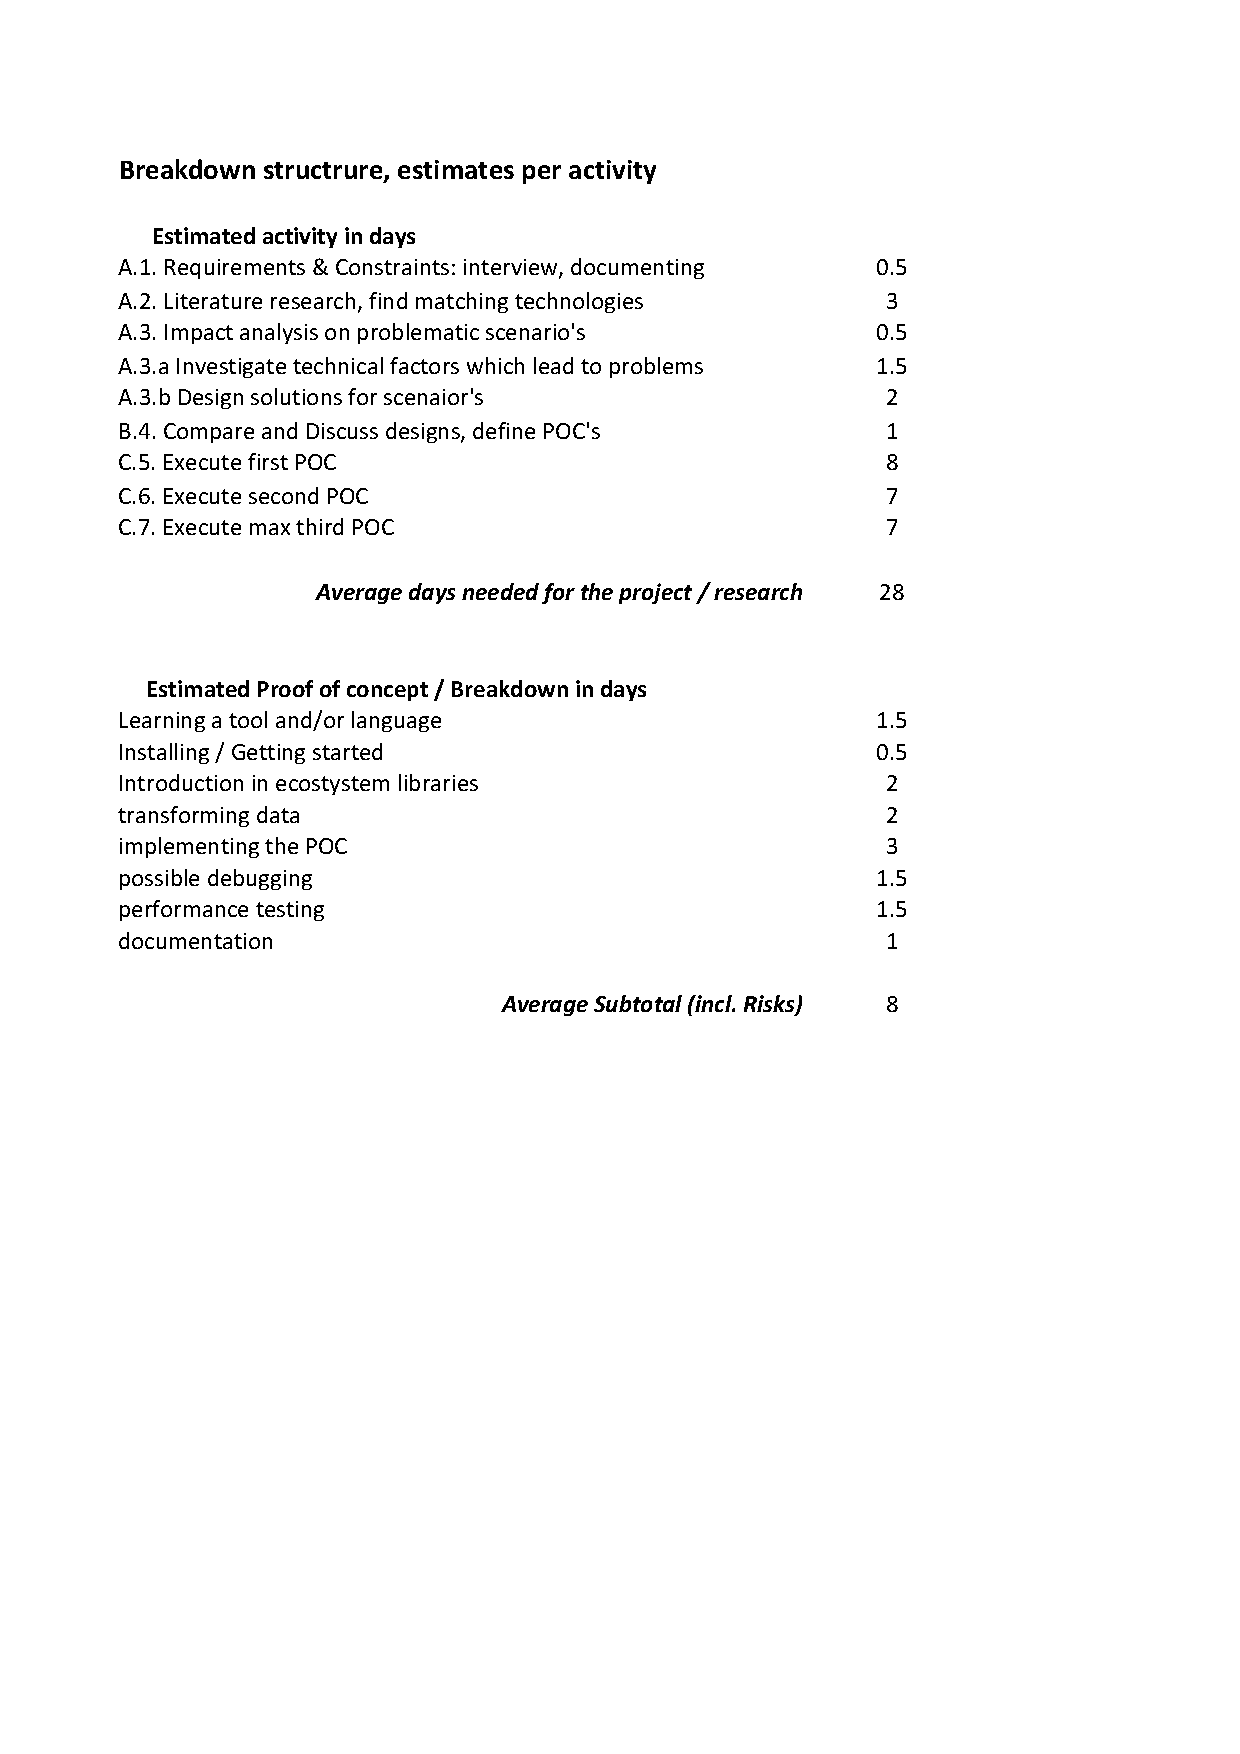
\includepdf[pages={1,2}]{appendix/planning-appendix-A.pdf}
